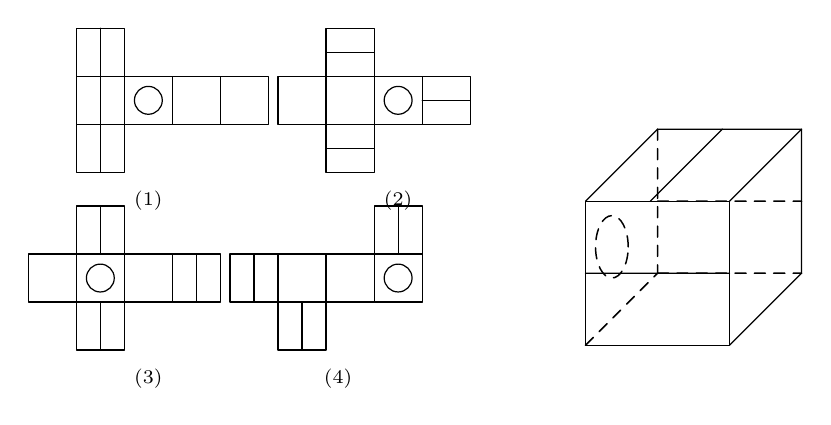
\begin{tikzpicture}[scale=.61, every node/.style={font=\scriptsize}, line cap=round, line join=round]
  \tikzset{face/.style={draw=black, line width=.44pt}, marker/.style={draw=black, line width=.44pt}, hidden/.style={draw=black, dash pattern=on 4pt off 3pt, line width=.54pt}}

  % (1): three vertical faces carry a vertical centre mark.
  \begin{scope}[shift={(0,3.7)}]
    \foreach \x/\y in {0/0,0/1,0/2,1/1,2/1,3/1} {
      \draw[face] (\x,\y) rectangle ++(1,1);
    }
    \draw[marker] (.5,0)--(.5,3);
    \draw[marker] (1.5,1.5) circle (.29);
    \node[below] at (1.5,-.18) {(1)};
  \end{scope}

  % (2): horizontal centre marks occur in the three indicated faces.
  \begin{scope}[shift={(5.2,3.7)}]
    \foreach \x/\y in {0/0,0/1,0/2,-1/1,1/1,2/1} {
      \draw[face] (\x,\y) rectangle ++(1,1);
    }
    \draw[marker] (0,.5)--(1,.5) (0,2.5)--(1,2.5) (2,1.5)--(3,1.5);
    \draw[marker] (1.5,1.5) circle (.29);
    \node[below] at (1.5,-.18) {(2)};
  \end{scope}

  % (3): vertical centre marks occur in the top, bottom, and far-right faces.
  \begin{scope}[shift={(0,0)}]
    \foreach \x/\y in {0/0,0/1,0/2,-1/1,1/1,2/1} {
      \draw[face] (\x,\y) rectangle ++(1,1);
    }
    \draw[marker] (.5,0)--(.5,1) (.5,2)--(.5,3) (2.5,1)--(2.5,2);
    \draw[marker] (.5,1.5) circle (.29);
    \node[below] at (1.5,-.18) {(3)};
  \end{scope}

  % (4): the top and bottom marked faces attach to different faces in the row.
  \begin{scope}[shift={(5.2,0)}]
    \foreach \x/\y in {-2/1,-1/1,0/1,1/1,1/2,-1/0} {
      \draw[face] (\x,\y) rectangle ++(1,1);
    }
    \draw[marker] (-1.5,1)--(-1.5,2) (1.5,2)--(1.5,3) (-.5,0)--(-.5,1);
    \draw[marker] (1.5,1.5) circle (.29);
    \node[below] at (.25,-.18) {(4)};
  \end{scope}

  % Cube: visible edges are solid; rear and lower-left edges, the ellipse, and
  % the two hidden horizontal marks use the original dashed convention.
  \begin{scope}[shift={(10.6,.1)}]
    \draw[face] (0,0)--(3,0)--(3,3)--(0,3)--cycle;
    \draw[face] (0,3)--(1.5,4.5)--(4.5,4.5)--(3,3);
    \draw[face] (3,0)--(4.5,1.5)--(4.5,4.5);
    \draw[marker] (0,1.5)--(3,1.5) (1.35,3)--(2.85,4.5);
    \draw[hidden] (1.5,4.5)--(1.5,1.5) (1.5,3)--(4.5,3) (1.5,1.5)--(4.5,1.5) (0,0)--(1.5,1.5);
    \draw[hidden] (.55,2.05) ellipse (.34 and .65);
  \end{scope}
\end{tikzpicture}
